\usection{Il Programma di Simulazione}

Dungeons \& Dragons è un \wargam{e} che parla di avventura e di narrativa avventurosa. Si versa un sacco di inchiostro su come il gioco sia eccitante ed eroico. Ai tempi, l'attenzione si concentrava su quanto il gioco fosse o non fosse realistico. Si dice fin troppo poco delle assunzioni sottostanti la simulazione del mondo, in particolare visto che \dnd{}, da questo punto di vista, è stranamente ambizioso per un \wargam{e}. Penso che ora possa valer la pena di guardare a che cos'è la cosa effettivamente interessante fatta dal gioco.

\usubsection{Cosa stiamo simulando?}

Il famoso sistema di livelli di personaggio di \dnd{} permette agli avventurieri di diventare più forti man mano che hanno successo nelle avventure, dedicandosi a nuove avventure più pericolose ed eccitanti. Perché? Non è strano che qualcuno diventi "più forte" per merito dell'"andare all'avventura"?

L'idea è spesso presentata come una modellazione dello sviluppo di abilità e l'esperienza nella carriera da parte del personaggio, qualcosa che ha poco senso quando guardi alla direzione generale delle regole. Se le regole simulano addestramento ed esperienza, per come effettivamente funzionano per gli esseri umani, lo fanno veramente male. Gli esseri umani diventano più traumatizzati, non più abili, man mano che vengono usati come sacco da boxe dai mostri.

Un brutto sottotono della questione viene portato dai chiari intenti di gamification introdotti dagli sviluppatori iniziali del gioco; Gary Gygax, per esempio, vide indubbiamente il potenziale di variare premi e penalità in stile gioco d'azzardo e più spesso che no preferiva (cinicamente, secondo me) l'intrattenimento all'illuminazione. Non sempre, l'uomo lottava chiaramente con la natura creativa dell'attività, il gioco sembra prendere fin troppo spesso forma dall'orribile convenienza della tirannia del divertimento. La risposta al perché i personaggi diventano più potenti col passare del tempo è che è il modo migliore di prenderti all'amo, tesoro.

Se questa fosse la miglior risposta alla domanda del programma simulativo di \dnd{}, il gioco non sarebbe meglio dell'infinità dei suoi discendenti videoludici. Una scatola di Skinner meccanica, che insegna ai giocatori a deliziarsi di monete d'oro immaginarie, mentre le distribuisce a velocità ottimizzate per la soddisfazione. Vedi crescere i numeri, una barra di progresso fa "ding!"; l'ottundente oppio della nostra era.

\usubsection{Un modello di narrativa eroica}

Mettendo da parte questa deprimente non-risposta, ecco la sostanza positiva che vedo in \dnd{}: il programma di studi del gioco come \wargam{e} si interessa al livello mutevole di \textbf{privilegio drammatico}: ci si aspetta che i personaggi di livello più alto modellino il modo in cui i protagonisti avventurosi di generi di narrativa d'avventura più ottimisti e stilizzati operino e si rapportino col mondo attorno a loro.

Con questa interpretazione, i personaggi giocanti iniziano al primo livello e avanzano verso i livelli superiori \textit{attraverso il successo nelle avventure} perché l'attività di gioco fa da prova e dimostra la natura di protagonista di un dato personaggio. Il gioco modella il protagonismo attraverso l'idea fantasiosa che possiamo scoprire chi sono gli eroi solo vedendo chi sopravvive ad avventure eroiche. Il tuo personaggio ottiene i vantaggi modellati di essere "l'eroe" come conseguenza dell'essere già sopravvissuto con successo a un'avventura eroica.

Qui è essenziale comprendere la distinzione tra un gioco che modelli la "statura eroica" del suo protagonista fittizio e uno che invece modelli come la trama di queste storie si sviluppi effettivamente. \dnd{} appartiene al primo tipo: il gioco dovrebbe fornire una distribuzione stocasticamente affidabile di esiti in sfide avventurose per eroi fittizi contrapposti pericoli avventurosi, usando una logica morbida per colmare le incertezze del modello. Il risultato non è una storia, ma semplicemente l'approssimazione simulata di "cosa succederebbe se", che solo coincidentalmente tiene conto di un eroismo ineffabile come uno dei suoi fattori.

Comprendere questo schema è una precondizione per poter davvero praticare il \wargam{ing} con lo scheletro di \dnd{}, poiché non puoi calibrare le meccaniche delle regole e prendere decisioni appropriate senza una chiara comprensione di ciò che stai modellando. Il \wargam{ing} vive di modellazione, quindi con un gioco dedicato a modellare la narrativa avventurosa \textit{pulp}, dovresti essere in grado di prendere un romanzo di \textsc{Doc Savage} e assegnare delle capacità meccaniche al personaggio in base al testo. Di che livello è Doc Savage? Questo è ciò che viene misurato dai livelli di \dnd{}, il livello di distinzione romantica, il genere in cui esiste l'eroe.

Una volta, quando il \wargam{ing} in \dnd{} era più popolare, questo era una specie di passatempo: discutere su quale fosse il livello appropriato a cui modellare, diciamo, Gandalf il Grigio o Conan il Barbaro. Riconosco tranquillamente di star presentando una teoria originale sull'argomento di \dnd{}, ma mi sembra di non essere il primo a battere questi sentieri.

\usubsection{La simulazione di base}

Prima di considerare il modo in cui il privilegio drammatico del protagonista viene rappresentato nelle regole del gioco, è necessario considerare la simulazione della realtà di base utilizzata da \dnd{}: il gioco offre un modello completo e semplice di come funziona il mondo fittizio sottostante quando i protagonisti drammatici sono altrove. Il privilegio drammatico opera contro questa struttura di base e ne trae il proprio valore.

Come ci si potrebbe aspettare, \dnd{} si occupa prima e soprattutto di guerra nei dungeon, quindi è quello di cui si occupa la base:

\textbf{Un umano normale} ha pochi punti ferita, circa 1d6. Questa manciata di punti è una risorsa astratta che protegge la persona dalle conseguenze negative dell'avventura. I punti si perdono durante l'avventura, recuperano secondo regole specifiche e, se li finisci, succedono cose brutte al personaggio. Ma finché i punti persistono, tutto va essenzialmente bene.

\textbf{Un pericolo avventuroso} causa una ferita misurata in punti ferita. Un nemico che colpisce un personaggio con una spada potrebbe causare 1d6 danni, quindi un ammontare piuttosto considerevole, se paragonato a quindi punti ferita potrebbe avere la vittima; il colpo potrebbe o meno rivelarsi traumatico. Similmente, altri pericoli causano danni ai PF, di più per i pericoli considerati più chiaramente pericolosi.

\textbf{Gettarsi in battaglia} per i combattenti di default (diciamo i soldati normali), è un affare confuso in cui, salvo armature e difese specifiche, chiunque ha circa il 50\% di possibilità di ferire il proprio avversario nell'arco di una singola unità temporale di mischia. Potrebbe succedere, potrebbe non succedere, ma se continui a provare prima o poi qualcuno si farà male. Altre manovre rischiose hanno probabilità similari di "potrebbe succedere, oppure no". Quando ci si fa male, vedi sopra per il consumo di punti ferita.

\textbf{I numeri salgono} per due ragioni distinte: o una data creatura è davvero sovrumana in qualche modo importante, come un ippopotamo è più grosso e più forte di un umano, o viene consdirata avere un'agenzia tematica superiore sotto forma di livelli. Entrambe queste casistiche hanno le loro basi dettagliate, da usare per creare le statistiche di un'immensa varietà di situazioni e di come si rapportano con le riserve di punti ferita.

Questo, dunque, è il cuore del \textbf{modello realistico di base} dell'interazione avventurosa in \dnd{}. Tremendamente semplice e piuttosto astratto, vero? Deve esserlo, perché il gioco elabora e decora partendo da questa base molto, molto oltre quello che ti aspetteresti sia possibile. Ma queste sono le basi.

Non posso sottolineare abbastanza l'importanza per un futuro arbitro di comprendere questa parte: quando ti serve sapere quanti danni fa un motore che cade su un meccanico, la risposta non è nel regolamento, ma è certamente nel modello simulativo: 1d6 punti è appropriato per minacce ordinarie e non sovrannaturali che hanno il potenziale di causare seri danni o morte, ma non la certezza di farlo.

\begin{figure}[p!]
    \resizebox{\linewidth}{!}{
        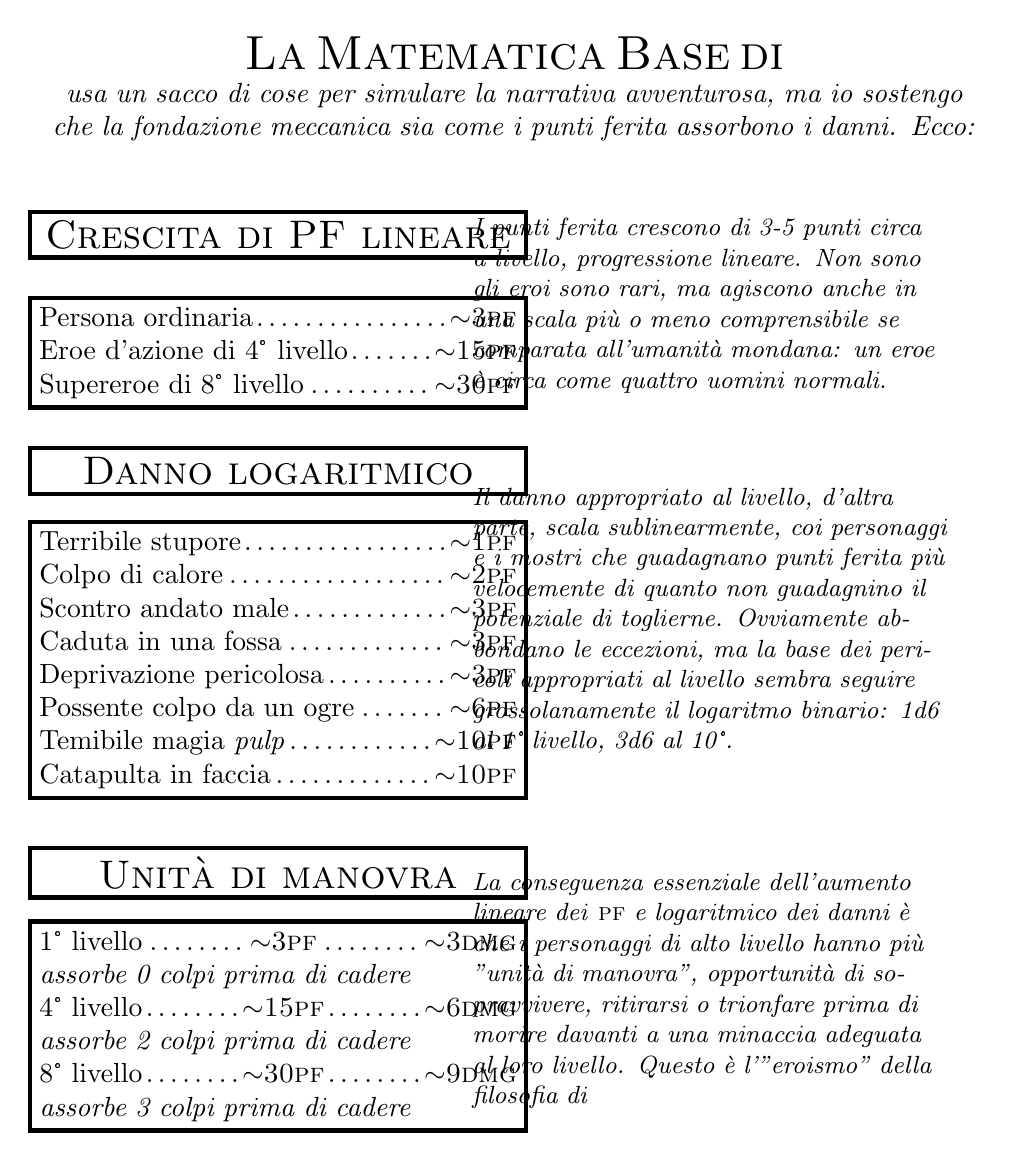
\begin{tikzpicture}
            \node[text width=\linewidth, align=center] (T) at (-1, 0.25) {
                    \textsc{\LARGE{La Matematica Base di \dnd{}}}\\
                    \dnd{} \textit{usa un sacco di cose per simulare la narrativa avventurosa, ma io sostengo che la fondazione meccanica sia come i punti ferita assorbono i danni. Ecco:}
                };

            \node[draw, ultra thick, rectangle,font=\Large\scshape,text width=0.5\linewidth,align=center] (A) at (-4, -1.6) {Crescita di PF lineare};
            \node[draw, ultra thick, rectangle, text width=0.5\linewidth] at (-4, -3.1) {
                Persona ordinaria\dotfill$\sim$\textsc{3pf}\\
                Eroe d'azione di 4° livello\dotfill$\sim$\textsc{15pf}\\
                Supereroe di 8° livello\dotfill$\sim$\textsc{30pf}
            };
            \node[rectangle, text width=0.5\linewidth, font=\itshape\small] at (1.5,-2.5) {I punti ferita crescono di 3-5 punti circa a livello, progressione lineare. Non sono gli eroi sono rari, ma agiscono anche in una scala più o meno comprensibile se comparata all'umanità mondana: un eroe è circa come quattro uomini normali.};
            
            \node[draw, ultra thick, rectangle,font=\Large\scshape,text width=0.5\linewidth,align=center] (A) at (-4, -4.6) {Danno logaritmico};
            \node[draw, ultra thick, rectangle, text width=0.5\linewidth] at (-4, -7) {
                Terribile stupore\dotfill$\sim$\textsc{1pf}\\
                Colpo di calore\dotfill$\sim$\textsc{2pf}\\
                Scontro andato male\dotfill$\sim$\textsc{3pf}\\
                Caduta in una fossa\dotfill$\sim$\textsc{3pf}\\
                Deprivazione pericolosa\dotfill$\sim$\textsc{3pf}\\
                Possente colpo da un ogre\dotfill$\sim$\textsc{6pf}\\
                Temibile magia \textit{pulp}\dotfill$\sim$\textsc{10pf}\\
                Catapulta in faccia\dotfill$\sim$\textsc{10pf}\\
            };
            \node[rectangle, text width=0.5\linewidth, font=\itshape\small] at (1.5,-6.5) {Il danno appropriato al livello, d'altra parte, scala sublinearmente, coi personaggi e i mostri che guadagnano punti ferita più velocemente di quanto non guadagnino il potenziale di toglierne. Ovviamente abbondano le eccezioni, ma la base dei pericoli appropriati al livello sembra seguire grossolanamente il logaritmo binario: 1d6 al 1° livello, 3d6 al 10°.};

            \node[draw, ultra thick, rectangle,font=\Large\scshape,text width=0.5\linewidth,align=center] (A) at (-4, -9.7) {Unità di manovra};
            \node[draw, ultra thick, rectangle, text width=0.5\linewidth] at (-4, -11.65) {
                1° livello\dotfill$\sim$\textsc{3pf}\dotfill$\sim$\textsc{3dmg}\\
                \textit{assorbe 0 colpi prima di cadere}\\
                4° livello\dotfill$\sim$\textsc{15pf}\dotfill$\sim$\textsc{6dmg}\\
                \textit{assorbe 2 colpi prima di cadere}\\
                8° livello\dotfill$\sim$\textsc{30pf}\dotfill$\sim$\textsc{9dmg}\\
                \textit{assorbe 3 colpi prima di cadere}

            };
            \node[rectangle, text width=0.5\linewidth, font=\small] at (1.5,-11.2) {\textit{La conseguenza essenziale dell'aumento lineare dei} \textsc{pf} \textit{e logaritmico dei danni è che i personaggi di alto livello hanno più "unità di manovra", opportunità di sopravvivere, ritirarsi o trionfare prima di morire davanti a una minaccia adeguata al loro livello. Questo è l'"eroismo" della filosofia di }\dnd{}};


        \end{tikzpicture}
    }
\end{figure}

\usubsection{La scala del livello drammatico}

Ci sono molte direzioni per elaborare come diverse circostanze di avventura ti portano a guadagnare o perdere punti ferita in un allegro girotondo di goduria ludica, ma quella più immediatamente rilevante per i giocatore è come gli avventurieri diventino più forti guadagnando "livelli". Salire di livello fondamentalmente impatta le regole che si applicano ai personaggi in modi che li rendono più capaci di comportarsi effettivamente come protagonisti dell'avventura. Il gioco suggerisce che cominci a giocare dalla base realistica e continui l'investigazione verso i reami sempre più estremi del fantasy avventuroso e romantico man mano che le tue abilità di gioco crescono.

Questo argomento viene esaminato troppo raramente nella cultura di \dnd{}, ed è un peccato, perché causa un sacco di confusione non necessaria su come dovrebbero andare le cose. Il fatto è che i personaggi di 1° livello, in \dnd{}, sono poveri bastardi fragili, che facilmente faranno fini terribili se osano andare all'avventura. Questo fa brillare i personaggi di alto livello come le gemme prezione che sono. Presentare \dnd{} come un gioco di baldanzoso eroismo è un disservizio al modo in cui copre i generi.

In termini pratici, ecco come l'aumento di livello e, conseguentemente, di PF si allinea ai generi letterari:

\paragraph{I personaggi di 1° livello, avventurieri di bassa lega da $\sim$3 punti ferita di protagonismo eroico} sono a malapena abbastanza importanti da avere un nome. Si troverebbero a loro agio in una storia di avventura realistica (spesso scritto "cinica"), del tipo in cui a volte i personaggi muoiono e non ci sono veri eroi. Sono tutti semplicemente persone che provano a sopravvivere. I thriller di guerra, crimine e spionaggio sono talvolta scritti a questo cupo e nichilistico livello di dettaglio anti-drammatico ma, seriamente, questo è quasi un modello della realtà (o quantomeno della comprensione della stessa che i giocatori portano al tavolo). Se questi avventurieri non insistessero a infilarsi il luoghi orribili per fare fini terribili potrebbero tranquillamente essere persone ordinarie.

\paragraph{I personaggi di 4° livello, eroi di media fascia, con $\sim$17 punti ferita in una confezione da eroe d'azione} sono confortevolmente eroici in quel modo da basso profilo che viene presentato dalla narrativa d'avventura: la storia non si sforza più di tanto per rappresentare l'eroe con un invulnerabile dio della guerra o qualcosa del genere, ma hanno abbastanza fortuna, destino e "plot armor" da rendere veramente ovvio chi è l'eroe e chi i comprimari.\\
Il grosso degli eroi della narrativa d'avventura, da Flash Gordon a Indiana Jones passando per Batman opera più o meno secondo queste regole da "livelli intermedi". La differenza meccanica fondamentale è che questi personaggi, se comparati con le persone normali, hanno un discreto ammontare di punti ferita di scorta, che li aiuta a sopravvivere ai rischi che corrono. E, ovviamente, alcune abilità piuttosto eccezionali.

\paragraph{I personaggi di 8° livello, supereroi di fascia alta, con un'emblematica prestanza sovrumana da $\sim$30 punti ferita} sono essenzialmente super uomini, le regole mutano e massaggiano la realtà in loro favore in infiniti modi. Le loro capacità rasentano una perfezione fantastica e, nel genere fantasy, controllano molte magie potenti. Questi personaggi appaiono all'estremità superiore della curva di potere della narrativa fantastica, ma è anche il livello in cui la narrativa fantastica inizia a diventare qualcosa di diverso. Le storie di supereroi o wuxia parlano forse meno di avventura (persone in pericoli emozionanti) e più di forze idealizzate in rotta di collisione. Qualsiasi cosa sia, \dnd{} si propone comunque di modellarlo.

\usubsection{Come la gomma tocca l'asfalto}

Potrei star ripetendo l'ovvio qui, ma, per essere completamente esplicito, questo è il modello tecnico fondamentale su cui la risoluzione delle azioni di \dnd{} riposa:\\
Pericolo! $\rightarrow$ Danno ai PF! \hfill$\rightarrow$ Il bastardo di 1° livello muore!

\hfill$\rightarrow$ L'eroe di 4° livello prosegue!

Vuoi regole per i pericoli (combattimenti o qualsiasi altra cosa) che permettano ai personaggi di manovrare tra un colpo e l'altro. Fai in modo che quella riserva di PF sia l'orologio di una minaccia. Questo è il modo in cui il gioco gestisce l'eroismo: dove un altro sarebbe caduto, l'eroe continua ad avanzare. La prima imboscata dei cattivi "li manca per fortuna" (sottrae punti ferita). Questo è il privilegio drammatico.

\usubsection{Un invito allo studio}

La cosa veramente bella del curriculum di studi suggerito dal gioco, avviare una campagna al 1° livello e sudarsi l'"avanzamento di livello" per entrare in nuovi tipi di narrativa avventurosa, è che è estremamente organico. Questi riferimenti rispetto ai quali un personaggio di 4° livello è "eroico" o cosa sono fondamentalmente proclamazioni \textit{top-dowm} di definizioni tautologiche: i personaggi crescono fino all'eroismo al proprio passo, l'ambientazione della campagna che li circonda segue le proprie regole e nel \dnd{} come \wargam{ing} non ci sono dietro le quinte su come le cose dovrebbero funzionare. Certo, prendi la tua compagnia di soldati umani regolari e attacca il Conte Dracula, vediamo come va a finire per voi; questo è esattamente il gioco progettato meticolosamente per rispondere a questo tipo di domande in maniera ragionata e giocabile. Sto caratterizzando un "eroe" come uno che ha 15 punti ferita dalla mia esperienza organica in gioco, non come richiesta.

L'idea di trovare una via d'uscita combattendo dal "Vietnam fantasy" e spostarsi poi nelle più ampie acque dell'avventura eroica non è, ovviamente, incisa nella pietra. Per ora, io raccomando di seguire il programma: è interessante proprio per la sua brutalità nel fissare le regole di base e definire la moneta dell'eroismo. Decisamente il punto d'ingresso raccomandato per il programma artistico di \dnd{}.

\usubsection{Le classi di personaggio nella simulazione}

Dando per assodato quanto detto prima, qual è quindi il ruolo della classe del personaggio nella simulazione della narrativa fantastica? Oltre a livelli e punti ferita, è questo il singolo concetto meccanico che si nota di più in \dnd{}.

Come per il livello del personaggio, io ovviamente non considero credibile trattare la classe del personaggio come un modello diegetico della sua occupazione o classe sociale; se fosse questo quello che sta modellando, lo starebbe facendo terribilmente male.

Sostengo, invece, che la classe del personaggio miri a modellare il privilegio protagonistico di uno specifico archetipo letterario. Ecco perché le classi dei personaggi sono generalmente basate sull'archetipo idealizzato di questo o quello specifico tipo di protagonista letterario e perché sono piene di regole specifiche su come quel tipo di personaggio rompa le normali regole del gioco nei diversi livelli (intensità delle eccezioni drammatiche).

Un modo possibilmente illuminante di pensare a come modellare qualcosa di così ineffabile e possibilmente soggettivo come il tema letterario dell'"eroismo" o, che è intercambiabile, il concetto di struttra narrativa di "essere un protagonista", nei termini perenni di \dnd{} di classe e livello: il tuo livello è il peso della tua influenza sul mondo di gioco, come una riserva d'acqua, e la tua classe è il canale attraverso cui detta influenza è liberata sul mondo. La classe del personaggio è l'affermazione che modella come, in una data campagna, si manifesta l'eroismo.

Con molte delle sue regole meccaniche semplici e orientate agli aspetti pratici, è qui che giace il grosso dell'attenzione del gioco: nel determinare che tipo di eroi possono esistere nell'ambientazione di gioco e come possano interagire col mondo e con sè stessi. Quando scegli quali classi esistono nel mondo della tua campagna, stai modellando il tipo di protagonismo drammatico che la campagna in questione accetta come reale.